\chapter{Módulo 1: Práticas corporais}

\coment{Este módulo tem o objetivo de o aluno identificar as principais
características das práticas corporais reconhecendo as modalidades que
são definidas como jogos, esportes, lutas, ginásticas e danças.\\
Habilidades BNCC: EF35EF03, EF35EF15.}

\colorsec{Habilidades Saeb}

\begin{itemize}
\item
  Identificar elementos constitutivos dos esportes, da ginástica e das
  lutas.
\item
  Identificar a importância do respeito ao oponente e às normas de
  segurança na vivência das práticas corporais (jogos, lutas,
  ginásticas, esportes e dança).
\item
  Analisar os esportes e as lutas nas suas manifestações profissional e
  de lazer.
\item
  Avaliar situações de preconceito no contexto das práticas corporais.
\item
  Avaliar meios para superar situações de preconceito no contexto das
  práticas corporais.
\end{itemize}

%\textless{}Arte: a ideia é fazer um mapa mental com os textos a seguir\textgreater{}

\conteudo{\textbf{Pratica corporal:} são todas ações que fazem com que o nosso
corpo se movimente para fazer uma simples tarefa do dia, realizar algum
exercício físico ou alguma modalidade esportiva.

\textbf{Esportes}: atividade voltada para competições que têm regras
fixas e que não podem ser alteradas. Também tem confederações que
fiscalizam os esportes e as competições.

\textbf{Danças}: atividade que o praticante usa o corpo para se
expressar por meio de passos de danças e que tem a presença de música.
Também é usada para diversão e socialização podendo ser realizada
individual, em dupla ou em grupos.

\textbf{Lutas}: Prática que foi criada para a defesa pessoal que tem
diferentes golpes (chutes, socos, técnicas de queda etc.). São práticas
que promove aspectos filosóficos ao praticante para evitar brigas.

\textbf{Ginástica}: prática que tem o objetivo de fortalecer o corpo por
meio de movimentos acrobáticos ou de exercícios físicos ajudando a saúde
e a qualidade podendo usar algum material (bolas, bastões, halteres,
máquinas etc.) ou apenas o próprio corpo.

\textbf{Jogos brincadeiras}: atividades que têm semelhanças com alguns
esportes e é voltada para o lazer e diversão. Sua principal
característica é que no jogo as regras podem ser modificadas. Podem
existir brincadeiras de diferentes culturas, como a indígena, africana
etc.}

\coment{É importante que os estudantes saibam
diferenciar e identificar cada tipo de prática corporal. É possível que
a turma entenda que tudo é esportes, mas muitas práticas corporais não
foram criadas para o aspecto de competição, e sim para diversão ou
saúde.}

\colorsec{Atividades}

\num{1} Escreva um exemplo de uma prática corporal.

\begin{enumerate}
\item
  Esporte: \coment{Futebol, handebol, vôlei.}
\item
  Lutas: \coment{Judô, karatê, boxe.}
\item
  Danças: \coment{Samba, tango, valsa, hip-hop.}
\item
  Ginásticas: \coment{Pilates, yoga, exercícios de musculação.}
\item
  Jogos e brincadeiras: \coment{Pega-pega, esconde-esconde.}
\end{enumerate}

\coment{As respostas são pessoais para cada
estudante, então pode aparecer outras respostas. Essa atividade tem como
objetivo analisar o conhecimento prévio deles e identificar se eles
sabem diferenciar cada prática corporal. Habilidade Saeb: Identificar
elementos constitutivos dos esportes, da ginástica e das lutas.}

\num{2} Qual a principal diferença entre um esporte, como o futebol, com um
  jogo, como a brincadeira do ``bobinho''?

\linhas{3}
\coment{Os esportes têm regras fixas e são voltadas para competições. Já os
jogos (brincadeiras) podem ter suas regras alteradas para promover a
diversão entre os praticantes. Habilidade Saeb: Identificar elementos
constitutivos dos esportes, da ginástica e das lutas.}

\num{3} Leia as afirmativas a seguir e marque V para as verdadeiras e F para
  as falsas.

\begin{boxlist}
\item As lutas ajudam as pessoas a brigarem. \coment{F}

\item As danças podem ajudar na socialização, mas podem ser realizadas individualmente. \coment{V}

\item As ginásticas dificilmente melhoram a qualidade de vida do praticante. \coment{F}

\item As brincadeiras podem ser adaptadas para cada grupo de pessoas. \coment{V}

\item Os esportes tem como função incentivar discussões entre as pessoas. \coment{F}
\end{boxlist}

\coment{Essa atividade deve ser usada para os
estudantes identificarem cada atividade prática. Caso seja necessário,
retome as principais características e exemplos das práticas corporais.
Habilidade Saeb: Identificar elementos constitutivos dos esportes, da
ginástica e das lutas.}

\num{4} Leia o texto a seguir e complete as lacunas com as palavras abaixo:

\begin{itemize}
\item Segurança 
\item Cuidados 
\item Respeitar 
\item Regras 
\item Prática
\end{itemize}

\begin{quote}
Não importa a \preencher\coment{prática} corporal, sempre devemos \preencher\coment{respeitar} as pessoas que
estão participando da atividade respeitando também as \preencher\coment{regras}. Além
disso, também devemos realizar os devidos \preencher\coment{cuidados} para que a atividade
prática seja realizada com \preencher\coment{segurança} para ninguém se machucar.
\end{quote}
\coment{Essa atividade vai ajudar o estudante a
entender que em qualquer prática corporal deve seguir as normas, ou
seja, as regras para promover a segurança e o respeito entre os
participantes. Habilidade Saeb: Identificar a importância do respeito ao
oponente e às normas de segurança na vivência das práticas corporais
(jogos, lutas, ginásticas, esportes e dança).}


\num{5} Imagine a seguinte situação: Um amigo da sua turma começou a praticar
  o hip-hop, mas alguns colegas falam que ele deve parar de dançar. O
  motivo é que falam que as danças só podem ser realizadas pelas
  meninas.

Com base nessa situação, podemos afirmar que tem um preconceito?
Justifique sua resposta.

\linhas{3}
\coment{Sim, pois o preconceito está no pensamento de achar que
algumas modalidades são exclusivas para meninas ou para meninos.}

\coment{Essa atividade vai ajudar o estudante a
entender situações preconceituosas que podem surgir nas práticas
corporais. Habilidade Saeb: Avaliar situações de preconceito no contexto
das práticas corporais.}

\num{6} Ligue as definições do lazer e da profissão com os exemplos das
  práticas corporais de lutas e de esportes.

\begin{multicols}{2}
Seguir as regras de uma competição oficial de judô. 

Brincar de esgrima com espadas de papel. 
 
Treinar de 6 a 8 horas por dia para uma partida importante. 

Jogar bola no parque com os amigos. 

\columnbreak

Profissão no esporte

Lazer no esporte

Profissão nas lutas

Lazer nas lutas
\end{multicols}

\coment{Essa atividade vai ajudar ao estudante a
entender que tanto o esporte, quanto as lutas podem ser realizadas no
âmbito profissional (realizar várias horas de treino, treinar para uma
competição e seguir regras etc.) ou para o lazer (diversão com amigos ou
família, adaptara regras e materiais). Habilidade Saeb: Analisar os
esportes e as lutas nas suas manifestações profissional e de lazer.}

\num{7} Na sua turma entrou uma colega nova que era de um outra escola, mas
  alguns colegas acabam excluído ela durante o recreio e em algumas
  atividades da escola. Sendo assim, escreva uma solução para fazer com
  que essa colega tenha amigos.

\linhas{3}
\coment{Uma solução é realizar jogos ou brincadeiras com a turma toda
para ajudar na socialização entre os colegas.}

\coment{Essa atividade tem como objetivo o aluno
analisar uma situação preconceituosa (excluir um colega na escola) e
encontrar uma solução para acabar com esse preconceito usando as
práticas corporais. Habilidade Saeb: Avaliar meios para superar
situações de preconceito no contexto das práticas corporais.}

\colorsec{Seção Treino}

\num{1} Leia o texto a seguir:

\begin{quote}
Conhecido entre os Xavante como tobdaé, essa é a brincadeira com a
peteca, palavra de origem Tupi que significa~``golpear com as mãos''.
Feita com areia, penas, couro ou palha de milho, na brincadeira o
desafio é tocar na peteca sem deixá-la cair no chão. Outra variante da
diversão é tentar acertar a peteca em outro jogador, que deve deixar a
partida se for acertado.

\fonte{6 brincadeiras indígenas para divertir crianças e aproximar culturas.
Centro de Referências em Educação Integral. Disponível em:
https://educacaointegral.org.br/reportagens/6-brincadeiras-indigenas-para-divertir-criancas-e-aproximar-culturas/.
Acesso em: 13 fev. 2023.}
\end{quote}

O texto mostra uma atividade para o lazer, pois a prática corporal indígena tem

\begin{escolha}
\item variações de como pode ser realizada.

\item movimentos com golpes de lutas.

\item regras que não podem ser alteradas.

\item materiais oficiais para a prática.
\end{escolha}

\coment{Saeb: Analisar os esportes e as lutas nas suas manifestações
profissional e de lazer.

BNCC: (EF35EF03)~Descrever, por meio de múltiplas linguagens (corporal,
oral, escrita, audiovisual), as brincadeiras e os jogos populares do
Brasil e de matriz indígena e africana, explicando suas características
e a importância desse patrimônio histórico cultural na preservação das
diferentes culturas.

A) Correta. O texto fala de uma prática corporal voltada pelo lazer, ou
seja, uma brincadeira que possui regras a adaptações para a diversão.

B) Incorreta. Por mais que o nome da brincadeira seja ``golpear com as
mãos'', tobdaé é uma brincadeira para o lazer e não uma luta.

C) Incorreta. O texto mostra duas variações (regras) que podem ser
modificadas para brincar.

D) Incorreta. O texto mostra como a peteca é feita, mas não são
materiais oficiais semelhantes aos esportes e sim adaptações.}

\num{2} Leia o texto a seguir que fala sobre a luta indígena:

\begin{quote}
{[}..{]} Huka Huka, arte marcial indígena genuinamente brasileira.
{[}...{]}

Frente a frente, e abaixados para protegerem as pernas, os oponentes
giram em forma circular e se enfrentam primeiro pelo olhar.
Posteriormente, agarram-se para ver quem consegue levantar o adversário
e levá-lo ao chão, encostando as costas no solo {[}...{]}

Como não há um juiz, são os próprios atletas que decidem pela vitória,
derrota ou empate: caso em que se soltam um do outro e nenhum dos dois é
derrubado. A vitória é recompensada pelo reconhecimento e respeito das
comunidades indígenas ao vencedor.

\fonte{Huka Huka, a luta corporal do Xingu, contribui para manter viva a
cultura indígena no Mato Grosso. Ministério dos Povos Indígenas.
Disponível em:
https://www.gov.br/funai/pt-br/assuntos/noticias/2022-02/huka-huka-a-luta-corporal-do-xingu-contribui-para-manter-viva-a-cultura-indigena-no-mato-grosso.
Acesso em: 13 fev. 2023.}
\end{quote}

Com base no texto, podemos afirmar que a huka-huka é uma luta, pois

\begin{escolha}
\item tem regras que podem ser alteradas durante a prática,

\item prioriza o ganhador da luta com prêmios.

\item incentiva as brigas entres os indígenas.

\item promove o respeito entre os lutadores.
\end{escolha}

\coment{Saeb: Identificar a importância do respeito ao oponente e às normas de
segurança na vivência das práticas corporais (jogos, lutas, ginásticas,
esportes e dança).

BNCC: (EF35EF15)~Identificar as características das lutas do contexto
comunitário e regional e lutas de matriz indígena e africana,
reconhecendo as diferenças entre lutas e brigas e entre lutas e as
demais práticas corporais.

A) Incorreta. A luta huka-huka tem regras e objetivos que não podem ser
modificados, ou seja, as regras sempre vão ser as mesmas.

B) Incorreta. O texto mostra que os lutadores ganham respeito e
reconhecimento, e não prêmios.

C) Incorreta. A luta huka-hula é uma manifestação corporal que não
promove a briga entres os praticantes, e sim a cultura indígena e o
respeito.

D) Correta. Por meio do texto é possível analisar que a luta não tem
juiz e os próprios lutadores reconhecem a vitória do outro. Portanto, é
um sinal de demostrar respeito com outro.}

\num{3} Leia o texto a seguir:

\begin{quote}
\textbf{Jogos dos Povos Indígenas}

O critério para a participação desses jogos é a força cultural das
etnias, considerando tradições, como a língua, a dança, os rituais, os
cantos, as pinturas corporais, o artesanato e os esportes tradicionais.
{[}...{]}

As lutas corporais são realizadas por homens e mulheres e o esporte está
inserido na cultura tradicional dos povos que o praticam: os povos
indígenas Xinguanos, Bakairis os Huka Hukas e os Xavantes, de Mato
Grosso.~{[}...{]}

{[}...{]} Os lutadores se ajoelham girando em círculo anti-horário
frente ao oponente, até se entreolharem e se agarrarem, tentando
levantar o adversário e derrubá-lo ao chão. Os Karajá do Tocantins já
possuem outro estilo, pois os atletas iniciam a luta em pé, se agarrando
pela cintura, até que um consiga derrubar o outro ao chão

\fonte{Jogos dos Povos Indígenas. Secretaria da Educação. Disponível em:
http://www.educacaofisica.seed.pr.gov.br/modules/conteudo/conteudo.php?conteudo=218.
Acesso em: 13 fev. 2023.}
\end{quote}

Após ler o texto, podemos concluir que as luta indígenas se tornaram um
esporte, pois

\begin{escolha}
\item são realizadas por diferentes etnias indígenas

\item estão presentes em uma competição oficial.

\item apresentam variações para iniciar a luta.

\item tem a presença de pinturas corporais.
\end{escolha}

\coment{Saeb: Analisar os esportes e as lutas nas suas manifestações
profissional e de lazer.

BNCC: (EF35EF15)~Identificar as características das lutas do contexto
comunitário e regional e lutas de matriz indígena e africana,
reconhecendo as diferenças entre lutas e brigas e entre lutas e as
demais práticas corporais.

A) Incorreta. O fato de diferentes etnias indígenas não faz com que as
lutas se tornem um esporte, apenas mostra como essas práticas corporais
são importantes para essa cultura.

B) Correta. Uma das principais característica de uma prática corporal
ser um esporte é que ela deve estar presente em uma competição esportiva
oficial, como os Jogos dos Povos Indígenas.

C) Incorreta. A luta ter diferentes formas de iniciar a luta (em pé ou
ajoelhado) não é uma definição do esporte, só mostra algumas versões
dessa luta.

D) Incorreta. As pinturas corporais é uma característica da própria
cultura indígena, e não dos esportes.}

\chapter{Modulo 2: Jogos e brincadeiras}

\coment{Este módulo tem o objetivo de o aluno reconhecer a importância dos jogos
e brincadeiras para o desenvolvimento social e físico da pessoa. Também
vai fazer com que ele conheça novas culturas, como a indígena e a
africana. O aluno também vai perceber que muitos jogos pré-depsortivos
servem como uma iniciação esportiva para alguns esportes.\\
Habilidades BNCC: EF35EF01, EF35EF06.}

\colorsec{Habilidades Saeb:}

\begin{itemize}
\item
  Identificar as brincadeiras e os jogos populares como patrimônio
  histórico-cultural.
\item
  Valorizar o patrimônio histórico representado pelas brincadeiras e
  jogos, com ênfase naqueles de origem indígena e africana.
\item
  Analisar o protagonismo do trabalho coletivo na vivência dos jogos
  populares e dos esportes.
\end{itemize}

\conteudo{Os jogos e brincadeiras que realizamos em casa ou na escola trazem
vários benefícios para as pessoas. Por exemplo, essas atividades podem
ser usadas para promover a participação de todos, ou seja, evitar que
algum colega seja excluído. Um outro benefício é: ajudar as pessoas a
realizar as habilidades motoras, como saltar, correr, rolar, arremessar.
Habilidades essenciais para que as pessoas possam realizar as tarefas
simples do dia a dia.

Além disso, muitas brincadeiras são utilizadas como uma iniciação
esportiva. Um exemplo é a brincadeira ``bobinho'' do futebol, que é uma
atividade que as pessoas treinam os passes do futebol.

Por fim, muitas brincadeiras são consideradas como um patrimônio
cultural do país. O motivo é que mutas brincadeiras, jogos ou brinquedos
foram criados na cultura africana ou indígena. Duas culturas fortemente
presentes no país. Portanto, conhecer uma brincadeira faz com que a
gente conheça um pouco de uma cultura diferente.}

%https://br.freepik.com/vetores-gratis/criancas-felizes-brincando-de-amarelinha-no-playground\_24558957.htm\#page=2\&query=brincadeira\&position=10\&from\_view=search\&track=sph
%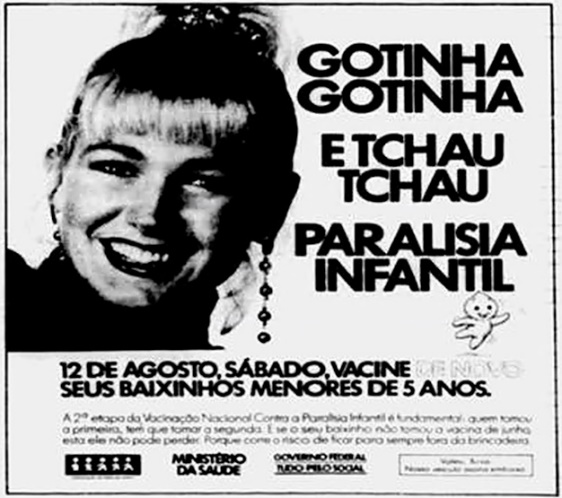
\includegraphics[width=3.39286in,height=1.88514in]{media/image2.jpeg}

\colorsec{Atividades}

\num{1} A seguir, tem algumas brincadeiras populares do Brasil. Escreva a cultura que representa cada brincadeira.

\begin{enumerate}
\item
  Cabo de guerra: \coment{Cultura indígena.}
\item
  Peteca: \coment{Cultura indígena.}
\item
  Mancala: \coment{Cultura africana.}
\item
  Terra-Mar: \coment{Cultura africana.}
\item
  Arco e flecha: \coment{Cultura indígena.}
\item
  Jogo da onça: \coment{Cultura indígena.}
\item
  Mamba: \coment{Cultura africana.}
\end{enumerate}

\coment{Caso seja necessário relembre os estudantes
de como as brincadeiras apresentadas são realizadas. Essa atividade tem
como objetivo de o estudante identificar origem de algumas brincadeiras.
Habilidade Saeb: Valorizar o patrimônio histórico representado pelas
brincadeiras e jogos, com ênfase naqueles de origem indígena e africana.}

\num{2} Um jogo popular em algumas escolas é o ``3 cortes''. Nesse jogo os
  participantes devem ficar passando a bola entre eles usando as mãos e
  no terceiro passe (toque) qualquer um pode dar uma cortada para tentar
  acertar alguém.

%https://br.freepik.com/vetores-gratis/um-menino-jovem-jogando-voleibol\_5284614.htm\#query=v\%C3\%B4lei\%20kids\&position=10\&from\_view=search\&track=ais
%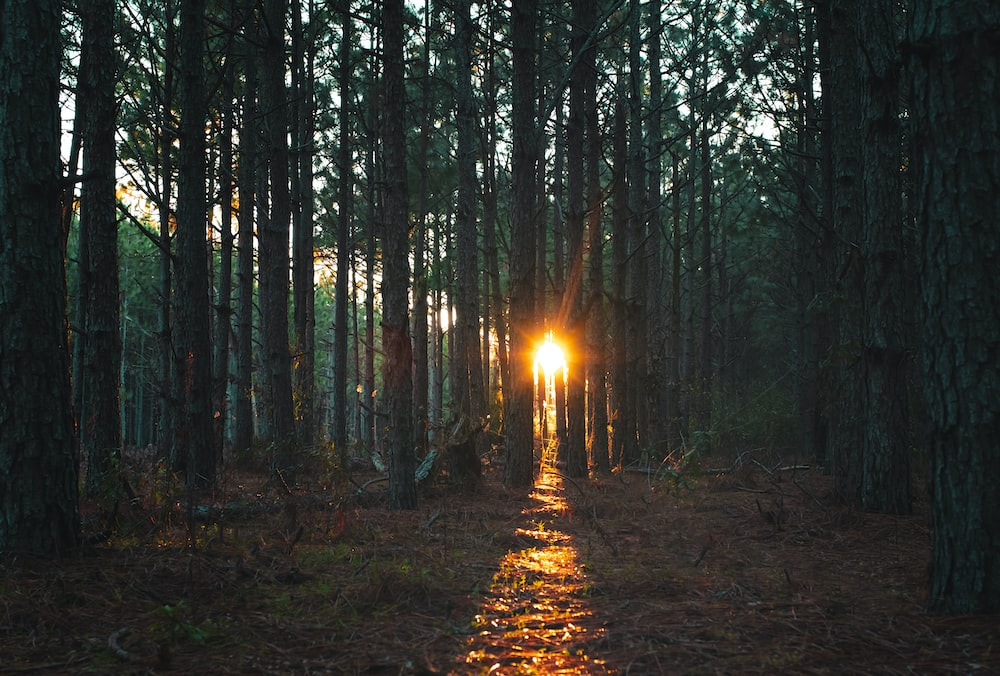
\includegraphics[width=1.29167in,height=2.20497in]{media/image3.jpeg}

Depois de ler o texto, a brincadeira apresenta características de qual
esporte? Justifique sua resposta.

\linhas{4}
\coment{A brincadeira ``3 cortes'' é um jogo pré-depsortivos do
voleibol pelo fato que nessa brincadeira os participantes realizam o
toque e a cortada. Dois fundamentos desse esporte.}

\coment{Os alunos podem escrever outros esportes
que usam a mão para jogar bola, como o basquete ou o handebol, mas a
brincadeira apresenta um fundamento do vôlei que é a cortada e o toque.
Habilidade Saeb: Identificar as brincadeiras e os jogos populares como
patrimônio histórico-cultural.}

\num{3} Uma brincadeira comum é a peteca, onde o objetivo é acetar esse objeto
  para que não encoste no chão. Existem vários tipos de petecas, mas foi
  criado pelos povos indígenas. Sendo assim, circule os materiais que
  esses povos usam para confeccionar a peteca.

%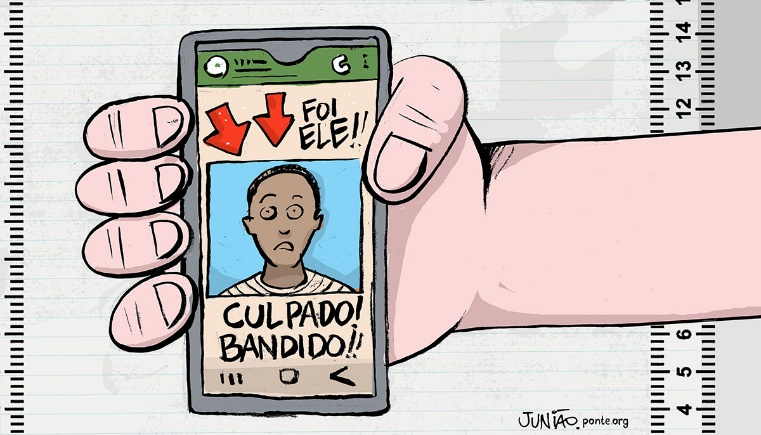
\includegraphics[width=1.84443in,height=1.22708in]{media/image4.jpeg}

\begin{multicols}{2}
\red{Borracha}

\red{Palha}

\red{Folhas}

\blue{Penas de animais}

\blue{Plástico}

\blue{Jornal}
\end{multicols}

\coment{Por meio dessa atividade o aluno vai
entender que muitos objetos usados na atualidade, como a peteca, podem
ser criados com elementos encontrados na natureza. Habilidade Saeb:
Valorizar o patrimônio histórico representado pelas brincadeiras e
jogos, com ênfase naqueles de origem indígena e africana.}

\num{4} Leia as afirmativas a seguir e marque V para as verdadeiras e F para
  as falas.

\begin{boxlist}
\item As brincadeiras podem fazer com que as pessoas sejam incluídas. \coment{V}

\item Uma vantagem das brincadeiras é fazer com que as pessoas trabalhem sozinhas. \coment{F}

\item Muitos jogos podem ser usados para aprender um novo esporte. \coment{V}

\item O trabalho em equipe pode ser usado em qualquer brincadeira. \coment{V}

\item O pega-pega é uma brincadeira que ajuda a nossa habilidade motora de rolar. \coment{V}
\end{boxlist}

\coment{Essa atividade tem o objetivo de o aluno
identificar outras vantagens de praticar uma brincadeira ou jogo
pré-depsortivos para promover a socialização e o trabalho em equipe.
Habilidade Saeb: Analisar o protagonismo do trabalho coletivo na
vivência dos jogos populares e dos esportes.}

\num{5} A seguir, é apresentado uma ilustração de bolinhas de gude. Uma
  brincadeira popular no Brasil, onde dependendo da região do país a
  maneira de brincar pode mudar. Até mesmo o nome da brincadeira pode
  mudar. Por exemplo, no Paraná é chamado de bola de búrica e em Alagoas
  é conhecido como ximbra.

%https://br.freepik.com/vetores-gratis/marbles\_797023.htm\#query=marbles\%20ball\&position=2\&from\_view=search\&track=ais
%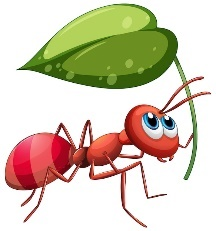
\includegraphics[width=2.04167in,height=2.04167in]{media/image5.jpeg}

Depois da leitura do texto, assinale a alternativa correta sobre a
brincadeira apresentada.

\begin{escolha}
\item
  As características das bolinhas de gude podem variar para cada região
  do país.
\item
  Somente no Sul do país que as bolinhas de gude são conhecidas.
\item
  As regras da brincadeira com bolinha de gude não podem mudar.
\item
  Dependendo do lugar as brincadeiras com bolinhas de gude apenas mudam
  de nome.
\end{escolha}

\coment{A resposta correta é a alternativa A. Por
meio dessa atividade o aluno vai analisar criticamente que muitas
brincadeiras podem mudar para cada região do país e por isso que muitas
atividades são populares no Brasil e por serem consideradas como um
patrimônio cultural do país por estar presente em muitas regiões do
país. Habilidade Saeb: Identificar as brincadeiras e os jogos populares
como patrimônio histórico-cultural.}

\colorsec{Seção Treino}

\num{1}
\begin{quote}
  {[}...{]} ensina o tag rugby, no qual as crianças usam um cinto com
  velcro do qual pende uma bandeirinha de tecido. Quando ela é retirada
  do adversário, ele tem que passar a bola, o que evita qualquer lance
  violento.

\fonte{Projeto busca popularizar rúgbi no país. Multi Rio. Disponível em:
https://www.multirio.rj.gov.br/index.php/reportagens/12329-projeto-busca-popularizar-r\%C3\%BAgbi-no-pa\%C3\%ADs.
Acesso em: 13 fev. 2023.}
\end{quote}

Com base no texto, a atividade prática citada tem o objetivo de

\begin{escolha}
\item desenvolver novos equipamentos esportivos.

\item diminuir brigas e conflitos nos esportes.

\item criar um novo esporte.

\item incentivar a prática de um espore.
\end{escolha}

\coment{Saeb: Analisar o protagonismo do trabalho coletivo na vivência dos jogos
populares e dos esportes.

BNCC: (EF35EF06)~Diferenciar os conceitos de jogo e esporte,
identificando as características que os constituem na contemporaneidade
e suas manifestações (profissional e comunitária/lazer).

A) Incorreta. O texto mostra que o praticante deve usar um cinto com
velcro com bandeirinha, mas o tag-rugby serve para popularizar o rugby e
não em criar novos equipamentos.

B) Incorreta. Por mais que o tag-rugby evita o contato físico, esse jogo
pré-desportivo tem o propósito de incentivar a pratica do rugby e não em
acabar com os conflitos nos outros esportes.

C) Incorreta. O tag-rugby não é um esporte e sim uma brincadeira do
rugby.

D) Correta. O texto mostra algumas variações do rugby para torna-lo mais
lúcio para as pessoas com o propósito de popularizar esse esporte.}

\num{2}

\begin{quote}
O mancala é um jogo de tabuleiro {[}...{]} mais antigo do mundo. É um
recurso lúdico utilizado pela Educação do Acre, em atividade
de~contraturno. {[}...{]}

O ato de semear, germinação das sementes na terra, desenvolvimento e
colheita são etapas no tabuleiro. Atualmente, é jogado em diversas
partes do mundo e possui mais de 200 variações.~``Mancala'' significa
mover.

\fonte{Mancala: Cultura africana apresentada de forma lúdica. Notícias do Acre.
Disponível em:
https://agencia.ac.gov.br/mancala-cultura-africana-apresentada-de-forma-ludica/.
Acesso em: 14 fev. 2023.}
\end{quote}

Por meio da brincadeira apresentada podemos

\begin{escolha}
\item adaptar a cultura para a nossa realidade.

\item aprender novas línguas.

\item conhecer tradições de diferentes locais do mundo.

\item estudar uma característica da cultura local.
\end{escolha}

\coment{Saeb: Valorizar o patrimônio histórico representado pelas brincadeiras e
jogos, com ênfase naqueles de origem indígena e africana.

BNCC: (EF35EF01)~Experimentar e fruir brincadeiras e jogos populares do
Brasil e do mundo, incluindo aqueles de matriz indígena e africana, e
recriá-los, valorizando a importância desse patrimônio histórico
cultural.

A) Incorreta. Porque são as regras do jogo mancala que podem ser
alteradas, e não a cultura africana.

B) Incorreta. Por mais que o texto mostra o significado da palavra
``mancala'', o jogo de tabuleiro não ensina novas palavras, e sim
apresenta um costume da cultura africana.

C) Correta. Por meio do texto podemos perceber que o mancal é um jogo
que representa a colheita da cultura africana, ou seja, por meio do jogo
de tabuleiro podemos conhecer diferentes tradições de outras culturas.

D) Incorreta. O texto mostra que o mancala é usado na escola, mas não
para que os alunos estudem um conteúdo relacionado a cultura local
(Acre), e sim sobre a cultura africana.}

\num{3}

\begin{quote}
Soltar pipa, jogar bola, pular amarelinha e brincar de pique-esconde
foram algumas das brincadeiras que se tornaram~Patrimônio Cultural do
Povo Carioca {[}...{]}

{[}...{]} que visem a~valorização e divulgação desta cultura, bem
como~oferecerá áreas específicas para que a prática dessas brincadeiras
possa continuar~ocorrendo na Cidade {[}...{]}

\fonte{Brincadeiras tradicionais viram Patrimônio Cultural do Povo Carioca;
veja a lista. G1. Disponível em:
https://g1.globo.com/rj/rio-de-janeiro/noticia/2021/11/05/brincadeiras-tradicionais-viram-patrimonio-cultural-do-povo-carioca-veja-a-lista.ghtml.
Acesso em: 14 fev. 2023.}
\end{quote}

Depois da leitura do texto, as brincadeiras citadas se tornaram um
patrimônio para que elas possam

\begin{escolha}
\item ser realizas em alguns lugares do país.

\item ter novas regras e variações.

\item incentivar a venda de materiais para brincar.

\item evitar com que as pessoas esqueçam dessas atividades.
\end{escolha}

\coment{Saeb: Identificar as brincadeiras e os jogos populares como patrimônio
histórico-cultural.

BNCC: (EF35EF01)~Experimentar e fruir brincadeiras e jogos populares do
Brasil e do mundo, incluindo aqueles de matriz indígena e africana, e
recriá-los, valorizando a importância desse patrimônio histórico
cultural.

A) Incorreta. O texto fala que os locais específicos para brincar é para
incentivar a pratica de algumas brincadeiras, e não para restringir as
brincadeiras tradicionais.

B) Incorreta. Porque o objetivo é preservar a cultura local por meio das
brincadeiras, e não de criar novas regras.

C) Incorreta. Porque o texto não cita que os locais voltados para as
brincadeiras vão incentivar o comércio, e sim incentivar as pessoas de
realizarem algumas brincadeiras tradicionais.

D) Correta. O texto mostra que algumas brincadeiras se tornarem um
patrimônio cultural e que vão ter locais para brincar com o objetivo de
as pessoas continuarem realizado as brincadeiras e preservando a cultura
local.}

\chapter{Modulo 3: Danças indígenas e africanas}

\coment{Este módulo tem o objetivo de o estudante relembrar as principias
características das danças, especialmente as de origens africanas e
indígenas, e identificar os elementos constitutivos da dança (ritmo,
espaço, gesto).\\
Habilidades BNCC: EF35EF09, EF35EF10, EF35EF11}

\colorsec{Habilidades Saeb:}

\begin{itemize}
\item
  Valorizar o patrimônio histórico representado pelas danças populares,
  com ênfase naquelas de matriz indígena e africana.
\item
  Comparar os elementos constitutivos de danças populares do Brasil e do
  mundo com aqueles de danças de matrizes indígena e africana.
\end{itemize}


\conteudo{As danças são práticas corporais que utiliza os movimentos do corpo para
se expressar e para se comunicar. Mesmo existindo diferentes tipos de
dança, todas elas têm três eleitos comuns que são:

\begin{itemize}
\item
  Ritmo: são as batidas fortes da música para que o dançarino possa
  realizar os movimentos de maneira coordenada e harmoniosa.
\item
  Espaço: é o local (trejeito) que o corpo realiza ao dançar dando a
  liberdade da pessoa se movimentar aonde ela quiser. É próprio para
  cada um.
\item
  Gesto: são os passos de dança que podem conter saltos, giros,
  movimentos acrobáticos. Os gestos podem ser padronizados, criados pelo
  próprio dançarino e podendo ser realizado em grupos ou
  individualmente.
\end{itemize}

É comum as pessoas conhecerem danças de outros lugares, como o tango, a
valsa etc., mas no Brasil existem muitas danças que surgiram no país,
como o samba, forró e assim por diante. Uma curiosidade é que no país
existem muitas danças de origem africana e indígena.

Também devemos saber que as danças trazem vários benefícios, como cuidar
da saúde e interagir com outras pessoas.}

%https://br.freepik.com/vetores-gratis/pacote-de-silhuetas-de-danca-de-silhuetas-de-dancarinas_23885929.htm\#query=dan\%C3\%A7a\&position=1\&from_view=search\&track=sph
%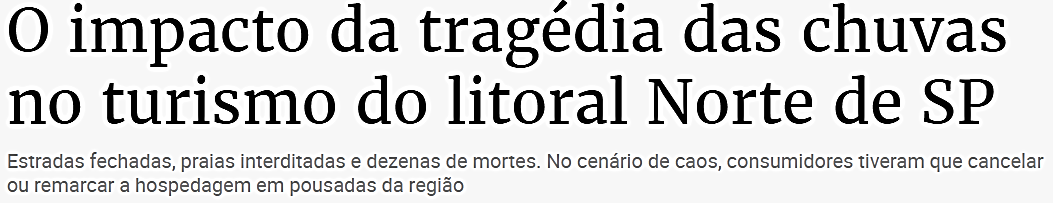
\includegraphics[width=4.58333in,height=1.53065in]{media/image6.png}

\colorsec{Atividades}

\num{1} Relacione as danças da primeira coluna com suas respectivas culturas de
  origem que estão na segunda coluna.

\begin{multicols}{2}
(\coment{2}) Toré
    
(\coment{2}) Kuarup
    
(\coment{1}) Samba

(\coment{1}) Cateretê

(\coment{2}) Maracatu

(\coment{1}) Maculelê

\columnbreak

(1) Cultura africana\medskip

(2) Cultura indígena
\end{multicols}

\coment{Essa atividade tem a finalidade do aluno
identificar e relembrar as danças que são das matrizes indígenas ou
africana. Habilidade Saeb: Valorizar o patrimônio histórico representado
pelas danças populares, com ênfase naquelas de matriz indígena e
africana.}

\num{2} Complete o texto a seguir com as palavras que estão faltando.

\begin{quote}
Não importa o tipo de dança, se é indígena, europeia ou africana, todas
elas têm algumas semelhanças!

Sabe aquelas batidas fortes que escutamos em uma música? Isso é o \preencher\coment{ritmo}.
Algo muito importante para que o dançarino consiga realizar o \preencher\coment{gesto} de
uma determinada dança. Por fim, o praticante também prestar atenção no
\preencher\coment{espaço} para que ele possa se movimentar na melhor maneira possível.
\end{quote}

\coment{A atividade serve como uma fixação para que
o estudante consiga identificar e diferenciar os três elementos
constitutivos da dança. Habilidade Saeb: Comparar os elementos
constitutivos de danças populares do Brasil e do mundo com aqueles de
danças de matrizes indígena e africana.}

\num{3} Observe a imagem e assinale V para as afirmativas verdadeiras e F para as falsas.

%
\includegraphics[width=2.71981in,height=2.00595in]{media/image7.jpeg}

\begin{boxlist}
\item A ilustração mostra o maculelê. \coment{V}

\item As pessoas da imagem estão realizando uma luta. \coment{F}

\item Uma característica é o uso de bastões de madeira. \coment{V}

\item A prática corporal apresentada é de origem indígena. \coment{F}
\end{boxlist}

\coment{Essa atividade vai ajudar o estudante a
reconhecer as principais características de uma dança de origem
africana. Habilidade Saeb: Valorizar o patrimônio histórico representado
pelas danças populares, com ênfase naquelas de matriz indígena e
africana.}

\num{4} Sabe qual é a dança mais popular no Brasil? Se pensou no samba, você
  acertou! É reconhecida internacionalmente como uma dança
  afro-brasileira e está presente em algumas festas populares no Brasil.
  Além disso, as pessoas se organizem em um grande círculo para dançar e
  tocar alguns instrumentos musicais, como o cavaquinho e o pandeiro.

%https://br.freepik.com/vetores-gratis/plano-de-fundo-do-carnaval-brasileiro\_3872754.htm\#query=samba\&position=8\&from\_view=search\&track=sph
%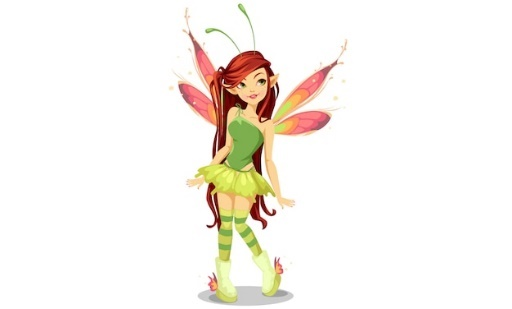
\includegraphics[width=3.13691in,height=3.13691in]{media/image8.jpeg}

Com base no texto, responda as questões a seguir:

\begin{escolha}
\item Porque o samba é conhecido como dança afro-brasileira?

\linhas{2}
\coment{O samba foi criado pelos negros escravizados que chegaram no Brasil e
que tem influencias da cultura brasileira.}

\item Em qual festa o samba é realizado?

\linhas{1}
\coment{Carnaval.}

\item Qual o nome da dança que as pessoas formam um círculo?

\linhas{1}
\coment{Samba de roda ou roda de samba.}
\end{escolha}

\coment{Por meio dessa atividade é possível o
estudante perceber como o samba está presente na cultura brasileira e
relembrar algumas características do samba. Habilidade Saeb: Valorizar o
patrimônio histórico representado pelas danças populares, com ênfase
naquelas de matriz indígena e africana.}

\num{5} Use o espaço abaixo para representar uma dança indígena e uma dança
  africana por meio de um desenho. Procure desenhar como são realizados
  os passos de dança, as vestimentas usadas e escreva o nome da dança
  que foi desenhada.

\begin{tabular}{l|l}
\hline
\textbf{Nome da dança indígena:} & \textbf{Nome da dança africana:} \\ \hline
\begin{tabular}[c]{@{}l@{}}\white{.}\\ \white{.}\\ \white{.}\\ \white{.}\\ \white{.}\end{tabular} & \begin{tabular}[c]{@{}l@{}}\white{.}\\ \white{.}\\ \white{.}\\ \white{.}\\ \white{.}\end{tabular} \\ \hline
\end{tabular}

\coment{Os desenhos elaborados pelos alunos vão
ajudá-los a a comparar as duas danças em relação aos gestos corporais.
Habilidade Saeb: Comparar os elementos constitutivos de danças populares
do Brasil e do mundo com aqueles de danças de matrizes indígena e
africana.}

\colorsec{Seção Treino}

\num{1}
\begin{quote}
  {[}...{]} \emph{toré}~apresenta variações de ritmos e toadas
  dependendo de cada povo. O~\emph{maracá}~-- chocalho indígena feito de
  uma cabaça seca, sem miolo, na qual se colocam pedras ou sementes --
  marca o tom das pisadas e os índios dançam, em geral, ao ar livre e em
  círculos. O ritual do~\emph{toré}~ é considerado o símbolo maior de
  resistência e união entre os índios
  do Nordeste brasileiro.

\fonte{Danças indígenas do Brasil. Fundação Joaquim Nabuco. Disponível em:
http://basilio.fundaj.gov.br/pesquisaescolar/index.php?option=com\_content\&view=article\&id=839:dancas-indigenas-do-brasil\&catid=39:letra-d.
Acesso em: 14 fev. 2023.}
\end{quote}

Assim como qualquer dança, a prática corporal indígena citada pode ser
considerada como uma dança pelo motivo de

\begin{escolha}
\item variar para cada povo indígena que existe no brasil.

\item ter instrumentos musicais para ditar o ritmo da dança.

\item ser realizado em locais abertos.

\item promover a interação entres os indígenas.
\end{escolha}

\coment{Saeb: Comparar os elementos constitutivos de danças populares do Brasil
e do mundo com aqueles de danças de matrizes indígena e africana.

BNCC: (EF35EF10)~Comparar e identificar os elementos constitutivos
comuns e diferentes (ritmo, espaço, gestos) em danças populares do
Brasil e do mundo e danças de matriz indígena e africana.

A) Incorreta. O fato do toré ser realizado por diferentes povos não quer
dizer que é uma dança, e sim uma prática que é difundida na cultura
indígena.

B) Correta. Porque o instrumento musical (maracá) serve para dar ritmo
na música e na dança, ou seja, é um elemento constitutivo da dança.

C) Incorreta. Porque a dança ser realizado ao ar livre não é uma
característica própria das danças.

D) Incorreta. Porque qualquer atividade promove a interação entre as
pessoas e não somente por meio das danças.}

\num{2}

\begin{quote}
Considerado, desde 2005, patrimônio cultural do Brasil pelo Iphan, o
  jongo conta agora com um centro cultural de 2 mil metros quadrados aos
  pés do Morro da Serrinha, em Madureira, zona norte do Rio. {[}...{]}

O jongo chegou ao Brasil com os escravos africanos de origem bantu,
vindos do Congo e de Angola, permanecendo presente entre aqueles que
trabalhavam nas lavouras de café e cana-de-açúcar no vale do Rio
Paraíba, entre São Paulo e Minas Gerais. Os proprietários das fazendas
permitiam que seus escravos dançassem jongo nos dias dos santos
católicos {[}...{]}

\fonte{Jongo, expressão da cultura afro-brasileira. Multi Rio. Disponível em:
https://www.multirio.rj.gov.br/index.php/reportagens/8637-jongo-expressao-da-cultura-afro-brasileira.
Acesso em: 14 fev. 2023.}
\end{quote}

Com base no texto, a dança apresentada é de origem africana, pois ela

\begin{escolha}
\item foi criada pelos negros escravizados.

\item surgiu no Sudeste do Brasil.

\item era praticada pelos fazendeiros de café.

\item estava relacionada com eventos religiosos.
\end{escolha}

\coment{Saeb: Valorizar o patrimônio histórico representado pelas danças
populares, com ênfase naquelas de matriz indígena e africana.

BNCC: (EF35EF09) Experimentar, recriar e fruir danças populares
do Brasil e do mundo e danças de matriz indígena e africana, valorizando
e respeitando os diferentes sentidos e significados dessas danças em
suas culturas de origem.

A) Correta. Porque o texto mostra que os negros escravizados, do Congo e
da Angola, que desenvolveram o jongo e por causa disso têm elementos
culturais africanos.

B) Incorreta. Porque o jongo tem influência da cultura africana do Congo
e da Angola, e não da cultura brasileira.

C) Incorreta. Porque eram os negros escravizados que trabalhavam nas
fazendas que realizavam a dança do jongo.

D) Incorreta. Por mais que a dança era praticada em ventos religioso,
isso foi criado no Brasil e não nos países africanos. Além disso, o
evento religioso não definia que a dança é de origem africana.}

\num{3}
\begin{quote}
O Samba de Roda no Recôncavo Baiano foi inscrito do Livro de Registro
das Formas de Expressão, em 2004. {[}...{]} a Unesco reconheceu esse
bem imaterial como Patrimônio Cutural Imaterial da Humanidade
{[}...{]}

{[}...{]} Atualmente, reúne as tradições culturais transmitidas por
africanos escravizados e seus descendentes, que incluem o culto aos
orixás e caboclos, o jogo da capoeira e a chamada comida de azeite. A
herança negro-africana no samba de roda se mesclou de maneira singular a
traços culturais trazidos pelos portugueses (principalmente viola e
pandeiro) e à própria língua portuguesa nos elementos de suas formas
poéticas.

\fonte{Samba de Roda do Recôncavo Baiano. IPHAN. Disponível em:
http://portal.iphan.gov.br/pagina/detalhes/56. Acesso em: 14 fev. 2023.}
\end{quote}

Depois da leitura do texto, a pessoa que pratica o samba vai

\begin{escolha}
\item realizar uma luta africana.

\item reconhecer costumes de origem europeia.

\item entender como uma atividade se torna um patrimônio.

\item conhecer diferentes culturais por meio da dança.
\end{escolha}

\coment{Saeb: Valorizar o patrimônio histórico representado pelas danças
populares, com ênfase naquelas de matriz indígena e africana.

BNCC: (EF35EF11)~Formular e utilizar estratégias para a execução de
elementos constitutivos das danças populares do Brasil e do mundo, e das
danças de matriz indígena e africana.

A) Incorreta. Porque o samba é voltado para a dança e não para praticar
a capoeira (luta africana).

B) Incorreta. Porque o samba é de origem africana e não europeia. Apenas
alguns instrumentos portugueses são usados, mas isso não faz com que o
praticante conheça a cultura europeia.

C) Incorreta. Porque o samba não tem o objetivo de o praticante entender
como a Unesco reconhecer uma atividade como patrimônio cultural.

D) Correta. Porque o texto mostra alguns elementos culturais presentes
no samba e por conta disso o praticante dessa dança vai poder conhecer
alguns costumes e tradições da cultura africana.}


\chapter{Simulado 1}

\num{1}
  %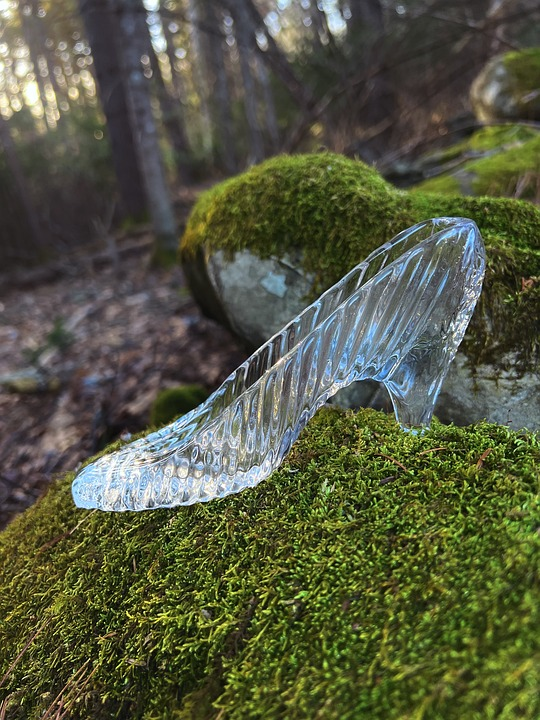
\includegraphics[width=2.17708in,height=1.39447in]{media/image9.jpeg}
%Disponível em: https://br.freepik.com/fotos-gratis/lutadores-de-karate-no-campeonato-de-luta-de-tatami\_30182444.htm\#query=jud\%C3\%B4\&position=42\&from\_view=search\&track=sph. Acesso em: 14 fev. 2023.

Observando os dois competidores, podemos perceber que eles estão
demostrando respeito para o outro. O motivo é que eles estão

\begin{escolha}
\item realizando uma saudação antes de lutar.

\item usando um kimono branco.

\item praticando a luta em uma competição.

\item evitando de usar golpes específicos das lutas.
\end{escolha}

\coment{Saeb: Identificar elementos constitutivos dos esportes, da ginástica e
das lutas.

BNCC: (EF35EF06)~Diferenciar os conceitos de jogo e esporte,
identificando as características que os constituem na contemporaneidade
e suas manifestações (profissional e comunitária/lazer).

A) Correta. Porque a saudação nas artes marciais ocidentais consiste em
inclinar o tronco para frente e mostrar o devido respeito ao adversário
antes de lutar.

B) Incorreta. Porque a vestimenta utilizada não é voltada para o
respeito e para simbolizar a paz.

C) Incorreta. Porque a competição não é um evento que promove o
respeito, e sim a competição.

D) Incorreta. Porque em competições os atletas devem usar técnicas da
luta para competir.}

\num{2}
\begin{quote}
  Os Jogos de Oposição {[}...{]} tem como característica o ato de
  confrontação que acontece entre duplas, trios ou até mesmo em grupos.
  Seus objetivos são vencer o adversário, impor-se fisicamente ao outro,
  respeito às regras e acima de tudo assegurar a segurança do colega
  durante as atividades.

Durante a aplicação dos Jogos de Oposição precisamos levar em
consideração alguns critérios de segurança para que não ocorram
acidentes. {[}...{]}

\fonte{Jogos de Oposição. Secretaria da Educação. Disponível em:
http://www.educacaofisica.seed.pr.gov.br/modules/conteudo/conteudo.php?conteudo=413.
Acesso em: 14 fev. 2023.}
\end{quote}

Com base no texto, as atividades práticas citadas são voltadas para
lutas, mas os participantes devem

\begin{escolha}
\item tentar ganhar de qualquer maneira.

\item tomar os devidos cuidados para ninguém se machucar.

\item realizar a atividade individualmente.

\item modificar as regras do jogo.
\end{escolha}

\coment{Saeb: Identificar a importância do respeito ao oponente e às normas de
segurança na vivência das práticas corporais (jogos, lutas, ginásticas,
esportes e dança).

BNCC: (EF35EF01)~Experimentar e fruir brincadeiras e jogos populares do
Brasil e do mundo, incluindo aqueles de matriz indígena e africana, e
recriá-los, valorizando a importância desse patrimônio histórico
cultural.

A) Incorreta. Porque o participante pode tentar a vitória desde que
respeite as regras e as normas de segurança.

B) Correta. Porque o próprio texto cita que os participantes devem
seguir as regras e normas de segurança para preservar a integridade
física do outro.

C) Incorreta. Porque o texto mostra que os jogos de oposição são
realizados em duplas ou em grupos.

D) Incorreta. Porque os participantes devem respeitar as regras e não as
mudar.}

\num{3}
\begin{quote}
  A Câmara analisa o Projeto de Lei 6933/10 {[}...{]} que regulamenta a
  profissão de instrutor de artes marciais. A proposta inclui na
  categoria os profissionais faixa preta que possuírem certificado de
  instrutor, monitor, professor ou 1° dan (graduação de arte marcial)
  emitido por uma federação ou associação registrada.

O certificado será concedido a quem comprovar a prática do esporte por
pelo menos dois anos e meio. Segundo o projeto, as federações e
associações criarão o código de ética dos profissionais e fiscalizarão o
cumprimento do período mínimo para obtenção do certificado.

\fonte{Proposta regulamenta profissão de instrutor de artes marciais. Agência
Câmara de Notícias. Disponível em:
https://www.camara.leg.br/noticias/143647-PROPOSTA-REGULAMENTA-PROFISSAO-DE-INSTRUTOR-DE-ARTES-MARCIAIS.
Acesso em: 14 fev. 2023.}
\end{quote}

Após a leitura do texto, o projeto de lei tem o objetivo de

\begin{escolha}
\item formar novos instrutores de lutas.

\item criar novas federações esportivas de lutas.

\item regulamentar a profissão de professores de lutas.

\item incentivar a prática de lutas.
\end{escolha}

\coment{Saeb: Analisar os esportes e as lutas nas suas manifestações
profissional e de lazer.

BNCC: (EF35EF06)~Diferenciar os conceitos de jogo e esporte,
identificando as características que os constituem na contemporaneidade
e suas manifestações (profissional e comunitária/lazer).

A) Incorreta. Porque o projeto de lei é para regulamentar soo
instrutores e não de ter novos profissionais.

B) Incorreta. Porque o objetivo é regulamentar os professores de lutas,
e não de criar novas entidades esportivas.

C) Correta. Porque no trecho ``... regulamenta a profissão de instrutor
de artes marciais...'' é possível analisar que o projeto de lei é
profissionalizar e regulamentar os instrutores de lutas.

D) Incorreta. Porque o objetivo é regulamentar os instrutores, e não
fazer com que mais pessoas pratiquem lutas.}

\chapter{Simulado 2}

\num{1}
\begin{quote}
  {[}...{]} no desenvolvimento da dança são encontrados vários
  descaminhos, entre eles estão os fatores que apontam para a exclusão
  da dança nos planejamentos de educação física {[}...{]}

{[}...{]} perguntamos se acham que exista algum preconceito dos alunos a
respeito do conteúdo dança {[}...{]} pedimos para dizer quais os
preconceitos encontrados, e 100\% deles responderam que o maior
preconceito está ligado ao gênero por parte dos meninos.

\fonte{O preconceito da dança nas escolas. Castro et. al. EFDeportes.com,
Revista Digital. Buenos Aires, Año 15, Nº 150, Noviembre de 2010.
Disponível em:
https://www.efdeportes.com/efd150/o-preconceito-da-danca-nas-escolas.htm.
Acesso em: 14 fev. 2023.}
\end{quote}

Com base no texto, o pensamento estereotipado na dança é achar que é um
(a)

\begin{escolha}
\item modalidade desconhecida por parte dos alunos.

\item esporte que é evitado na escola.

\item atividade que os homens não podem participar.

\item prática corporal voltada para mulheres.
\end{escolha}

\coment{Saeb: Avaliar situações de preconceito no contexto das práticas
corporais.

BNCC: (EF35EF09)~Experimentar, recriar e fruir danças populares do
Brasil e do mundo e danças de matriz indígena e africana, valorizando e
respeitando os diferentes sentidos e significados dessas danças em suas
culturas de origem.

A) Incorreta. Porque os alunos conhecem algumas danças, mas alguns não
preferem praticar essa modalidade.

B) Incorreta. Porque a dança pode ser sim ensinada na escola, mas é uma
prática que tem alguns preconceitos.

C) Incorreta. Porque os homens podem participar, mas existem alguns
pensamentos que acham que a dança é exclusiva para as mulheres.

D) Correta. Com no trecho ``... 100\% deles responderam que o maior
preconceito está ligado ao gênero por parte dos meninos...'' é possível
analisar que os meninos acreditam que as danças são para apenas um
gênero, ou seja, para o gênero feminino.}

\num{2}
\begin{quote}
  Acontece na próxima sexta-feira {[}...{]} no Ginásio Municipal de
  Esportes Domingos Angelino Régis, no Centro de Navegantes, um evento
  direcionado aos alunos das 8ª Séries da Rede Municipal de Ensino, que
  tem por objetivo despertar nos estudantes a importância do esporte
  como mecanismo de motivação, superação e combate ao preconceito. O
  evento também vai contar com a participação de atletas do paradesporto
  e da Apae de Navegantes.

{[}...{]} no local haverá uma apresentação das equipes de Basquete e
Handebol do Clube Roda

\fonte{Alunos participam de evento sobre motivação e superação através do
esporte. Prefeitura de Navegantes. Disponível em:
https://www.navegantes.sc.gov.br/noticia/9274/alunos-participam-de-evento-sobre-motivacao-e-superacao-atraves-do-esporte.
Acesso em: 15 fev. 2023.}
\end{quote}

O evento citado para os alunos serviu para que eles

\begin{escolha}
\item praticassem novos esportes.

\item promovessem a inclusão dos paratletas.

\item entendessem os benefícios dos esportes.

\item ajudassem na organização do evento.
\end{escolha}

\coment{Saeb: Avaliar meios para superar situações de preconceito no contexto
das práticas corporais.

BNCC: (EF35EF06)~Diferenciar os conceitos de jogo e esporte,
identificando as características que os constituem na contemporaneidade
e suas manifestações (profissional e comunitária/lazer).

A) Incorreta. Porque o evento serviu para combater o preconceito, e não
para apresentar novos esportes.

B) Incorreta. Porque foram os paratletas que deram palestras no vento
para os alunos falando sobre a inclusão no esporte.

C) Correta. Porque no trecho ``... esporte como mecanismo de motivação,
superação e combate ao preconceito...'' é possível analisar as vantagens
e benefícios que os esportes podem proporcionar.

D) Incorreta. Porque não foram os alunos que organizaram o evento e sim
os paratletas e a prefeitura local.}

\num{3}
\begin{quote}
  {[}...{]} caso das cantigas de roda que, historicamente fazem parte
  das tradicionais brincadeiras infantis {[}...{]}

{[}...{]} Ficou claro que a cantiga de roda é inserida em sala de aula
para promover o lúdico para a criança. {[}...{]} Nem todas as crianças
sabem cantar muitas músicas que são tidas como tradicionais. Isso porque
o envolvimento das mesmas com tecnologias pode estar afastando-lhes de
tradições ricas e importantes como são as cantigas de roda.

\fonte{As cantigas de roda como manifestações do patrimônio cultural: o papel
da escola na perpetuação dessa cultura. Patrimônio, Direitos Culturais e
Cidadania. Disponível em:
https://publica.ciar.ufg.br/ebooks/eipdcc-propostas-pratica-acoesdialogicas/artigos/artigo34.html.
Acesso em: 15 fev. 2023.}
\end{quote}

Com base no texto podemos perceber que a brincadeira tradicional citada

\begin{escolha}
\item está sendo esquecida por parte dos alunos.

\item vem ganhando popularidade por causa da tecnologia.

\item apresenta algumas desvantagens para os estudantes.

\item aparece como uma atividade pouco usada na escola.
\end{escolha}

\coment{Saeb: Identificar as brincadeiras e os jogos populares como patrimônio
histórico-cultural.

BNCC: (EF35EF01)~Experimentar e fruir brincadeiras e jogos populares do
Brasil e do mundo, incluindo aqueles de matriz indígena e africana, e
recriá-los, valorizando a importância desse patrimônio histórico
cultural.

A) Correta. Porque o texto mostra que algumas crianças não sabiam cantar
algumas cantigas tradicionais.

B) Incorreta. Porque é a tecnologia que está afastando as crianças das
cantigas populares.

C) Incorreta. Porque as cantigas trazem muitas vantagens e benefícios
aos alunos por ser algo lúdico.

D) Incorreta. Porque as cantigas são atividades que são sempre usadas no
ambiente escolar.}

\chapter{Simulado 3}

\num{1}
\begin{quote}
  Existem muitos jeitos de brincar, mas o objetivo é sempre desfrutar o
  momento e a companhia dos amigos. Além disso, os jogos ajudam a
  desenvolver habilidades que serão importantes ao longo da vida.
  Brincar é também uma maneira de aprender!

Os índios possuem muitos jogos e brincadeiras. Alguns são bastante
conhecidos por vários povos indígenas {[}...{]} como a peteca e a perna
de pau.

\fonte{Brincadeiras. Mirim Povos Indígenas Brasil. Disponível em:
https://mirim.org/pt-br/como-vivem/brincadeiras. Acesso em: 16 fev.
2023.}
\end{quote}

Segundo o texto, algumas brincadeiras indígenas

\begin{escolha}
\item são parecidas com algumas brincadeiras tradicionais.

\item são realizadas exclusivamente pelos indígenas.

\item são padronizadas para os povos indígenas.

\item são praticas de maneira individual.
\end{escolha}

\coment{Saeb: Valorizar o patrimônio histórico representado pelas brincadeiras e
jogos, com ênfase naqueles de origem indígena e africana.

BNCC: \textbf{(}EF35EF01)~Experimentar e fruir brincadeiras e jogos
populares do Brasil e do mundo, incluindo aqueles de matriz indígena e
africana, e recriá-los, valorizando a importância desse patrimônio
histórico cultural.

A) Correta. Porque as brincadeiras citadas (peteca e perna de pau) são
brincadeiras tradicionais de origem indígenas que muitas pessoas
conhecem.

B) Incorreta. Porque as brincadeiras de origem indígenas também são
realizadas por outros povos e cultura.

C) Incorreta. Porque no trecho ``...Existem muitos jeitos de
brincar...'' é possível analisar que existem variações nas brincadeiras.

D) Incorreta. Porque no trecho ``...o objetivo é sempre desfrutar o
momento e a companhia dos amigos...'' podemos compreender que as
brincadeiras são realizadas em grupo para promover a socialização.}

\num{2}
\begin{quote}
  {[}...{]} as crianças aprendem a respeitar o próximo, a ceder, a
  ganhar e a perder e constroem o senso de coletividade. Isso vai
  refletir no convívio com a família, na escola e, futuramente, até no
  trabalho.

\fonte{Esporte coletivo promove o respeito ao próximo e o trabalho em equipe.
G1 Bem estar. Disponível em:
https://g1.globo.com/bemestar/noticia/2016/08/esporte-coletivo-promove-o-respeito-ao-proximo-e-o-senso-de-coletividade.html.
Acesso em: 16 fev. 2023.}
\end{quote}

Com base no texto, podemos perceber que que o texto fala sobre

\begin{escolha}
\item os jogos pré-depsortivos.

\item os esportes competitivos.

\item as modalidades olímpicas.

\item as atividades escolares.
\end{escolha}

\coment{Saeb: Analisar o protagonismo do trabalho coletivo na vivência dos jogos
populares e dos esportes.

BNCC: (EF35EF06)~Diferenciar os conceitos de jogo e esporte,
identificando as características que os constituem na contemporaneidade
e suas manifestações (profissional e comunitária/lazer).

A) Correta. Porque os jogos são atividades voltadas para a diversão e
socialização.

B) Incorreta. Porque esportes competitivos visam apenas as competições e
as vitórias.

C) Incorreta. Porque, assim como os esportes, as modalidades olímpicas
visam o alto rendimento e as competições.

D) Incorreta. Porque o texto fala sobre jogos pré-depsortivos e não
sobre atividades escolares.}

\num{3}
  %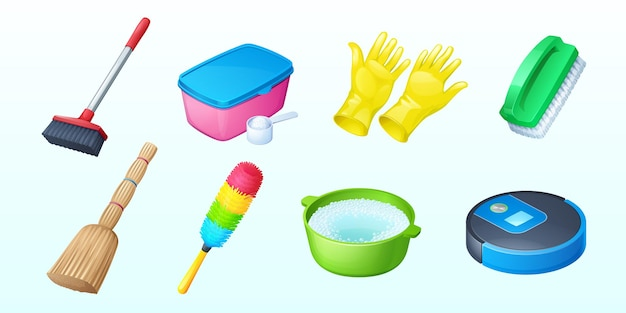
\includegraphics[width=3.43180in,height=2.28571in]{media/image10.jpeg}
%Disponível em: https://br.freepik.com/fotos-gratis/dancarinas-nigerianas-de-tiro-medio\_16130625.htm\#\&position=34\&from\_view=collections. Acesso em: 16 fev. 2023.

Observando a imagem, podemos perceber que é uma dança, pois

\begin{escolha}
\item as pessoas estão dançando ao ar livre.

\item as pessoas estão realizando uma pratica corporal coletiva.

\item as pessoas estão com vestimentas e pinturas corporais da dança.

\item as pessoas estão se movimentando no ritmo do batuque do instrumento
musical.
\end{escolha}

\coment{Saeb: Comparar os elementos constitutivos de danças populares do Brasil
e do mundo com aqueles de danças de matrizes indígena e africana.

BNCC: (EF35EF10)~Comparar e identificar os elementos constitutivos
comuns e diferentes (ritmo, espaço, gestos) em danças populares do
Brasil e do mundo e danças de matriz indígena e africana.

A) Incorreta. Porque as danças podem ser realizadas em espaço aberto ou
fechado e isso não define se uma atividade é uma dança oficial ou não.

B) Incorreta. Porque a dança pode ser realizada individualmente ou em
duplas. O fato de dança em grupo não define que uma pratica seja
considerada uma dança.

C) Incorreta. Porque as vestimentas e pinturas não são próprias da
dança, em vista que nos esportes, ginásticas e lutas podem ter essas
características.

D) Correta. Porque a pessoa se movimentado na batida da música
(instrumento musical) vai estar realizando o elemento constitutivo do
ritmo e do gesto da dança.}

\chapter{Simulado 4}

\num{1}
\begin{quote}
  Semba:~é uma dança de salão angolana urbana. Dançada em pares, com
  passadas distintas dos cavalheiros, seguidas pelas damas em passos
  totalmente largos, onde o malabarismo dos cavalheiros conta muito para
  o nível de improvisação. O Semba caracteriza-se como uma dança de
  passadas. Não é ritual nem guerreira, mas de divertimento,
  principalmente em festas.

\fonte{Danças Africanas. Secretaria da Educação do Estado do Paraná. Disponível
em:
http://www.educacaofisica.seed.pr.gov.br/modules/conteudo/conteudo.php?conteudo=62.
Acesso em: 16 fev. 2023.}
\end{quote}

Depois de ler o texto, prática corporal apresentada tem uma semelhança
com o samba. O motivo é que as duas danças são

\begin{escolha}
\item realizadas no carnaval.

\item originárias da cultura africana.

\item atividades competitivas.

\item praticadas em eventos religiosos
\end{escolha}

\coment{Saeb: Valorizar o patrimônio histórico representado pelas danças
populares, com ênfase naquelas de matriz indígena e africana

BNCC: (EF35EF11)~Formular e utilizar estratégias para a execução de
elementos constitutivos das danças populares do Brasil e do mundo, e das
danças de matriz indígena e africana.

A) Incorreta. Porque é apenas o samba que é realizado no carnaval.

B) Correta. Porque o samba se originou do semba, ou seja, as duas
surgiram com base nas influências culturas da África.

C) Incorreta. Porque as duas danças não são voltadas para as
competições.

D) Incorreta. Porque o samba e o semba não são danças religiosas.}

\num{2}
\begin{quote}
  O Governo do Paraná vai levar as artes marciais para dentro das
  escolas estaduais, oferecendo treinamentos no contraturno às aulas
  convencionais {[}...{]}

A ideia, explicou o governador {[}...{]} ``Gosto muito do esporte, sou
um praticante. As artes marciais ensinam a filosofia do respeito, a
obedecer a hierarquia, a ser uma pessoa do bem'' {[}...{]}

Além da introdução de artes marciais nas escolas estaduais, há outra
iniciativa que diz respeito ao Japs Combat, espécie de Jogos Abertos do
Paraná, voltado apenas para as artes marciais.

\fonte{Paraná vai levar as artes marciais para dentro das escolas. Agência
Estadual de Notícias. Disponível em:
https://www.aen.pr.gov.br/Noticia/Parana-vai-levar-artes-marciais-para-dentro-das-escolas.
Acesso em: 16 fev. 2023.}
\end{quote}

Depois de ler a reportagem, o objetivo das artes marciais é

\begin{escolha}
\item ensinar valores éticos aos alunos.

\item incentivar competições.

\item formar novos atletas.

\item aumentar os conflitos entre os alunos.
\end{escolha}

\coment{Saeb: Identificar a importância
do respeito ao oponente e às normas de segurança na vivência das
práticas corporais (jogos, lutas, ginásticas, esportes e dança).

BNCC: (EF35EF15)~Identificar as características das lutas do contexto
comunitário e regional e lutas de matriz indígena e africana,
reconhecendo as diferenças entre lutas e brigas e entre lutas e as
demais práticas corporais.

A) Correta. Porque no trecho ``... As artes marciais ensinam a filosofia
do respeito...'' mostra que as lutas ensinam o valor ético de respeitar
o outro.

B) Incorreta. Porque o objetivo das lutas é ensinar valores éticos e
morais, e não criar novas competições.

C) Incorreta. Porque o projeto apresentado serve para tornar os alunos
em cidadãos do bem.

D) Incorreta. Porque é justamente ao contrário que as lutas fazem. Elas
evitam e amenizam as brigas entre as pessoas.}

\num{3}
\begin{quote}
  {[}...{]} Por volta de 1880, jogadores de um clube inglês improvisaram
  um novo jogo por causa do mau tempo. Sobre uma mesa de sinuca, com
  livros como raquetes, um barbante como rede e uma bola de tênis
  normal, surgiram as primeiras raquetadas do tênis de mesa.

Encarado como brincadeira no começo, o desenvolvimento da modalidade
começou com regras bem similares às do tênis de quadra. O grande passo
dado pelo esporte veio em 1890, com a introdução da bola de celulóide,
perfeita para a prática do esporte. A partir dali, o tênis de mesa
começou a dar passos mais largos rumo à modernização.

\fonte{Tênis de mesa. Rede do Esporte. Disponível em:
http://rededoesporte.gov.br/pt-br/megaeventos/olimpiadas/modalidades/tenis-de-mesa.
Acesso em: 16 fev. 2023.}
\end{quote}

Com base no texto, o tênis de mesa antes de ser um esporte olímpico era

\begin{escolha}
\item uma atividade adaptada do tênis de campo.

\item uma modalidade esportiva.

\item um treinamento para usar as raquetes.

\item uma prática corporal para competição.
\end{escolha}

\coment{Saeb: Analisar os esportes e as
lutas nas suas manifestações profissional e de lazer.

BNCC: (EF35EF06)~Diferenciar os conceitos de jogo e esporte,
identificando as características que os constituem na contemporaneidade
e suas manifestações (profissional e comunitária/lazer).

A) Correta. Porque no começo as pessoas adaptaram alguns materiais para
simular as rebatidas na bola realizadas no tênis de campo.

B) Incorreta. Porque o texto cita que antes o tênis de mesa era uma
brincadeira.

C) Incorreta. Porque não era um treinamento, e sim uma brincadeira.

D) Incorreta. Porque o tênis de mesa antigamente era voltada para o
lazer.}

